% \documentclass[11pt]{article}
% \usepackage[margin=3cm]{geometry}
% \usepackage{xcolor}
% \usepackage{xcoffins}
% \usepackage{graphicx}

\documentclass[
    lang=en, 
    class=article,
    classOption={11pt},
    toc={redef}
]{zlatex}
\usepackage{xcoffins}
\zlatexColorSetup{
    link=teal
}
\usepackage{minted}
\usepackage{tcolorbox}
\tcbuselibrary{minted, breakable, skins}
\tcbset{listing engine=minted}
\definecolor{bg}{RGB}{242, 242, 242}
\newtcblisting{code}[1][latex]{
    enhanced,
    breakable,
    listing only, 
    minted language=#1, 
    minted style=manni,
    colback=bg, 
    frame hidden, 
    left=1mm, right=1mm,
    top=0mm, bottom=0mm, 
    minted options = {  
        autogobble,
        tabsize=2,
        breaklines=true, 
        breakanywhere=true,
        breakanywheresymbolpre=,
        breaksymbolleft=,
        fontsize=\footnotesize
    }
}
\usepackage{csquotes}

\title{Coffin Usage}
\author{Eureka}
\date{\today}
\begin{document}
\pagestyle{fancy}
\maketitle
\tableofcontents
\bigskip

\ExplSyntaxOn
\newcommand{\cmd}[1]{ \texttt{\tl_to_str:n {#1}}}
\newcommand{\usecoffin}[1]{\fbox{\TypesetCoffin #1}}
\newcommand{\pp}{\par\vspace*{2em}}
\ExplSyntaxOff
\section{introduce}
Current interfaces of \texttt{xcoffins} package is stable, See more at \TeX{} SE\footnote[1]{https://tex.stackexchange.com/a/397835/294585}

\subsection{What is Coffin}
coffin is a box not only containing ``something you type'', but also includes 
some information about it, like ``size, shape''.

Then we can \textbf{align 2 or more coffins}. How doese this archieve ? ``coffins''
privides a series of `poles(lines)' to connect some typical points on a coffin. We call these 
special points a ``handles''. Then 2 coffins can be align be describing the relationship between 
a handle on one confin with a handle a handle on the second.


\subsection{handles}
Handle positions are different in horizontal mode and vertical mode, next we consider coffin 
in horizontal mode. The following special handles are pre-defined: 
\begin{itemize}
    \item (hc, vc): center of a conffin
    \item (hc, t): horizontal center and top
    \item $\cdots$ 
\end{itemize}

we can simply remeber these handles by: \textbf{(right=r, horizontal center=hc, right=r)},
and \textbf{(top=t, vertical center=vc, bottom=b)}. You can see \cmd{(hc, vc)} contains 
2 lines \cmd{line-1=hc, line-2=vc}, then this point is the intersection.

Aside from pre-defined handles, each time you add a poles, (maybe) there will be some new handles 
added to this coffin. That's ``handles of a coffin is dynamic''.


\section{create and use coffins}
let's begin with a simple example: before align any 2 coffins, you must:
\begin{itemize}
    \item create a coffin (not local)
    \item add contents to this coffin
\end{itemize}

All coffin operations are local to current \TeX{} group. Decaler a coffin using
\cmd{\NewCoffin<\mycoffin>}, \cmd{\mycoffin} is the name of this new coffin.

Then we can add content to \cmd{\mycoffin}, the content add to this coffin can be typset in 
2 modes 
\begin{itemize}
    \item \cmd{\SetHorizontalCoffin\mycoffin{<your content>}}(\textbf{you can't line-break in this coffin(box)})
    \item \cmd{\SetVerticalCoffin\mycoffin{<width>}{<your content>}}
\end{itemize}

the the standard poles are set up based on the size of your content. Then you can use \cmd{\mycoffin}
using command \cmd{\TypesetCoffin\mycoffin} or \cmd{\usebox{\mycoffin}}(Legacy in \TeX{}).

\NewCoffin\mycoffin
\NewCoffin\myvcoffin
\SetHorizontalCoffin\mycoffin{i add something in this coffin, and this coffin is in horizontal mode. }
\SetVerticalCoffin\myvcoffin{10em}{i add something in this coffin, and this coffin is in vertical mode.}

\pp\usecoffin{\mycoffin}
\pp\usecoffin{\myvcoffin}


\subsection{coffin poles}
some standard poles list below:
\begin{itemize}
    \item \textbf{l}: left-hand edge
    \item $\cdots$
    \item \textbf{H}: a pole running along the \textbf{baseline} of the typeset material contained in the coffin
\end{itemize}

some extra poles in vertical mode material:
\begin{itemize}
    \item \textbf{B}: a pole running along the \textbf{baseline} of the material at the \textbf{bottom} of the coffin
    \item \textbf{T}: a pole running along the \textbf{baseline} of the material at the \textbf{top} of the coffin.
\end{itemize}



\subsection{set poles}
You can add some horizontal or vertical line a exist coffin, use the command (take \cmd{\mycoffin} for example):
\begin{itemize}
    \item \cmd{\SetHorizontalPole\mycoffin{<pole>}{<offset>}}. \cmd{<pole>} will be located at the \cmd{<offset>} 
        from the \textbf{baseline} of the coffin.
    \item \cmd{\SetVerticalPole\mycoffin{<pole>}{<offset>}}. \cmd{<pole>} will be located at the \cmd{<offset>} 
        from the \textbf{left-hand} edge of the bounding box of the coffin.
\end{itemize}

\SetHorizontalPole\mycoffin{height/3}{\TotalHeight/3}

You should notice that 
\[
    \mbox{Total height of coffin(base to top)} 
    = \mbox{\cmd{\TotalHeight}}  
    = \mbox{\cmd{\Height}}  + \mbox{\cmd{\Depth}}  
\]

\subsection{rotate coffin}
Use command \cmd{\RotateCoffin<coffin>{<angle>}} to ratate \textbf{counter-clockwise} about a \textbf{referance point}.
This process will rotate both the coffin content and poles. Use the above \cmd{\myvcoffin} for example, by command 
\cmd{\RotateCoffin\myvcoffin{45}} will result in:

\pp\RotateCoffin\myvcoffin{45}
\usecoffin{\myvcoffin}
\RotateCoffin\myvcoffin{-45}

Multiple rotations will not result in the bounding box of the coffin growing, it is just the bounding box become slope.

\subsection{scale coffin}
\subsubsection{absolute values}
If you are not satisfied with your coffin, you can resize it(scale to a fixed dimension in width or length), redefine 
its \cmd{<width>, <height>}. For that the coffin \cmd{\mycoffin} can't line-break, so the \cmd{<height>} is fixed. 
I'll use \cmd{\myvcoffin}. command \cmd{\ResizeCoffin\myvcoffin{4em}{2em+6em}} will result in:


% bugsin coffin copy: change tempcoffin will chenge original coffin in return.
% \pp\let\tempcoffin\myvcoffin
\pp\NewCoffin\tempcoffin
\SetVerticalCoffin\tempcoffin{10em}{i add something in this coffin, and this coffin is in vertical mode.}
\usecoffin{\tempcoffin}\hspace*{6em}
\ResizeCoffin\tempcoffin{4em}{2em+6em}
\usecoffin{\tempcoffin}

\subsubsection{scale factors}
To scale both length and with by given real numbers(factors) in $x$ and $y$ directions, use 
command \cmd{\ScaleCoffin<coffin>{<x-scale>}{<y-scale>}}. command \cmd{\ScaleCoffin\myvcoffin{2}{1}}
will result in:


\pp\NewCoffin\tempIIcoffin
\SetVerticalCoffin\tempIIcoffin{10em}{i add something in this coffin, and this coffin is in vertical mode.}
\usecoffin{\myvcoffin}\hspace*{6em}
\ScaleCoffin\tempIIcoffin{2}{1}
\usecoffin{\tempIIcoffin}

\cmd{\ResizeCoffin} and \cmd{\ScaleCoffin} can be used interchangeably, depend upon the context.



\subsection{join coffin}
Join coffin is one of the most important in operations of coffins. \cmd{xcoffins} provides 2 command for 
joining coffins: \cmd{\JoinCoffins, \JoinCoffins*}. The difference between these two is that: the first one 
will expand the bounding box of ``parent coffin'' while the ``child coffin'' will protrude outside of the 
bounding box of the updated ``parent coffin''.

How do these 2 coffins align (attacked)? 
\begin{itemize}
    \item First you select 2 \cmd{<handles>} in each of coffins, decaler these \cmd{<handles>}
        by intersection of 2 lines, that's \cmd{[<coffin1-pole1>, <coffin1-pole2>]}. 
    \item Second, after the 2 \cmd{<handles>} are setted up, align the 2 coffins by assingn the 
        \cmd{(x-offset>, <y-offset>)} to align these 2 coffins.
\end{itemize}

see figure (\ref{fig:join-coffins}).
\begin{figure}[!htb]
    \centering
    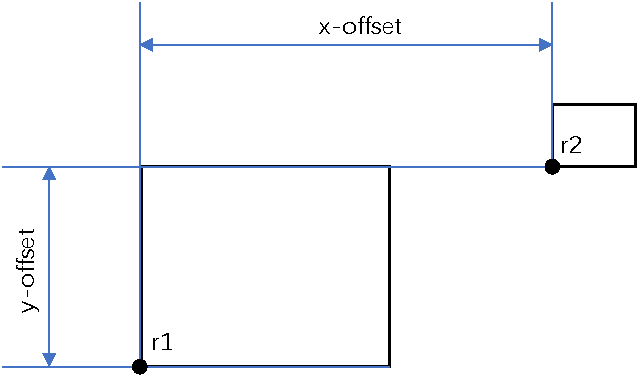
\includegraphics[width=.65\linewidth]{join_coffins.pdf}
    \caption{how to join coffins}
    \label{fig:join-coffins}
\end{figure}

So the full command to align 2 coffins is 
\begin{code}[latex]
\JoinCoffins
    <coffin1> [<coffin1-pole1>, <coffin1-pole2>]
    <coffin2> [<coffin2-pole1>, <coffin2-pole2>]
    (<x-offset>, <y-offset>)
\end{code}

Notice that ``This \cmd{<offset>} is an optional argument, and if it is not given then \cmd{(0pt, 0pt)} is used.''
When \cmd{\JoinCoffins} is used the new bounding box is the smallest rectangle containing the bounding boxes of the two 
input coffins. This may introduce addtional white space in this new ``bounding box'' when you rotate the joined (two) 
coffin(unless one coffin entirely overlaps the other).

Like applying ``\cmd{RortateCoffin}'' to a single coffin, Rotation of coffins will take account of the extent of the material 
after rotation when re-calculating the bounding box. This means that \textbf{no unnecessary white space} will be added on 
rotation as well.

The poles of the two input coffins are preserved within the structure of the updated coffin, consisting the original 
``poles'' in \textbf{both} coffins.

A simple joining operations as follows, the full code is:
\begin{code}[latex]
\def\bb#1{\color{#1!20!white}\rule{0.2 in}{0.2 in}}
% create coffins
\NewCoffin\OutputCoffin
\NewCoffin\RedCoffin
\NewCoffin\BlueCoffin
\NewCoffin\GreenCoffin
\NewCoffin\YellowCoffin
\NewCoffin\OrangeCoffin

% set coffins
\SetHorizontalCoffin\OutputCoffin{}
\SetHorizontalCoffin\RedCoffin{\bb{red}}
\SetHorizontalCoffin\BlueCoffin{\bb{blue}}
\SetHorizontalCoffin\GreenCoffin{\bb{green}}
\SetHorizontalCoffin\YellowCoffin{\bb{yellow}}
\SetHorizontalCoffin\OrangeCoffin{\bb{orange}}

% set coffins poles
\SetHorizontalPole\RedCoffin{red-vc}{\Height/2}
\SetVerticalPole\RedCoffin{red-hc}{\Width/2}
\SetHorizontalPole\BlueCoffin{blue-vc}{\Height/2}
\SetVerticalPole\BlueCoffin{blue-hc}{\Width/2}
\SetHorizontalPole\GreenCoffin{green-vc}{\Height/2}
\SetVerticalPole\GreenCoffin{green-hc}{\Width/2}
\SetHorizontalPole\YellowCoffin{yellow-vc}{\Height/2}
\SetVerticalPole\YellowCoffin{yellow-hc}{\Width/2}
\SetHorizontalPole\BlueCoffin{blue-t}{\Height}
\SetVerticalPole\BlueCoffin{blue-r}{0pt}

% join coffin to '\OutputCoffin'
\JoinCoffins\OutputCoffin[vc, hc]\RedCoffin[vc, hc]
\JoinCoffins\OutputCoffin[red-vc, red-hc]\BlueCoffin[l, b]
\JoinCoffins\OutputCoffin[blue-vc, blue-hc]\GreenCoffin[l, b]
\JoinCoffins\OutputCoffin[green-vc, green-hc]\YellowCoffin[l, b]
\JoinCoffins\OutputCoffin[blue-t, blue-r]\OrangeCoffin[r, b]

% typset the \OutputCoffin
\usecoffin{\OutputCoffin}
\end{code}


This code will result in the following graph:
\def\bb#1{\color{#1!20!white}\rule{0.2 in}{0.2 in}}
% create coffins
\NewCoffin\OutputCoffin
\NewCoffin\RedCoffin
\NewCoffin\BlueCoffin
\NewCoffin\GreenCoffin
\NewCoffin\YellowCoffin
\NewCoffin\OrangeCoffin

% set coffins
\SetHorizontalCoffin\OutputCoffin{}
\SetHorizontalCoffin\RedCoffin{\bb{red}}
\SetHorizontalCoffin\BlueCoffin{\bb{blue}}
\SetHorizontalCoffin\GreenCoffin{\bb{green}}
\SetHorizontalCoffin\YellowCoffin{\bb{yellow}}
\SetHorizontalCoffin\OrangeCoffin{\bb{orange}}

% set coffins poles
\SetHorizontalPole\RedCoffin{red-vc}{\Height/2}
\SetVerticalPole\RedCoffin{red-hc}{\Width/2}
\SetHorizontalPole\BlueCoffin{blue-vc}{\Height/2}
\SetVerticalPole\BlueCoffin{blue-hc}{\Width/2}
\SetHorizontalPole\GreenCoffin{green-vc}{\Height/2}
\SetVerticalPole\GreenCoffin{green-hc}{\Width/2}
\SetHorizontalPole\YellowCoffin{yellow-vc}{\Height/2}
\SetVerticalPole\YellowCoffin{yellow-hc}{\Width/2}
\SetHorizontalPole\BlueCoffin{blue-t}{\Height}
\SetVerticalPole\BlueCoffin{blue-r}{0pt}

% join coffin to '\OutputCoffin'
\JoinCoffins\OutputCoffin[vc, hc]\RedCoffin[vc, hc]
\JoinCoffins\OutputCoffin[red-vc, red-hc]\BlueCoffin[l, b]
\JoinCoffins\OutputCoffin[blue-vc, blue-hc]\GreenCoffin[l, b]
\JoinCoffins\OutputCoffin[green-vc, green-hc]\YellowCoffin[l, b]
\JoinCoffins\OutputCoffin[blue-t, blue-r]\OrangeCoffin[r, b]

% typset the \OutputCoffin
\usecoffin{\OutputCoffin}



\subsection{Typset Coffin}
How to typset a coffin we have decalered before, use command $\cmd{\TypsetCoffin}$. Though we have use this 
command before, but we haven't introduce the full syntax of this command. The full syntax is:

\begin{code}[latex]
\TypesetCoffin
    <coffin> [<pole1>, <pole2>]
    (<x-offset>, <y-offset>)
\end{code}

we can typset a coffin such that the relation between the \textbf{current reference point in docuemnt} and 
the \cmd{<handle>}(defined by these 2 lines) is described by the \cmd{<x-offset>} and \cmd{<y-offset>}.
Typesetting a coffin is therefore analogous to carrying out an alignment where the “parent” coffin is the 
current insertion point.


Finally, i'll introduce some functions measuring coffins, which is useful in \cmd{<dimension expression>}.


\section{Measuring Coffins}
\texttt{xcoffins} provide some function to measure the \cmd{depth, length, width} of a coffin. See below:
\begin{itemize}
    \item \cmd{\CoffinDepth<coffin>}: the depth of the coffin
    \item \cmd{\CoffinHeight<coffin>}: the height of the coffin
    \item \cmd{\CoffinTotalHeight<coffin>}: the total height of the coffin
    \item \cmd{\CoffinWidth<coffin>}: the width of the coffin
\end{itemize}

\section{Diagnostic}
Diagnostic data for following the coffin-building process is available both graphically and
at the terminal. 

Firstly, how to print a coffin including all the `poles' and `handles' in it? Use command
\cmd{\DisplayCoffinHandles<coffin>{<color>}}. This command will print the coffin with all the poles and
handles \textbf{graphically} at the current location in the source:

\pp
\DisplayCoffinHandles\myvcoffin{red}
\pp

It's also possible to show a specific \cmd{<handle>} by 2 poles you defiend before. Then introduce some 
Diagnostic functions in terminal, \cmd{\ShowCoffinStructure}. Using this function, you may see something like 
the below, command \cmd{\ShowCoffinStructure\myvcoffin}:
\begin{code}[latex]
Size of coffin \myvcoffin:
> ht = 34.80417pt
> dp = 0.0pt
> wd = 109.50027pt
Poles of coffin \myvcoffin:
>  l  =>  {0.0pt}{0.0pt}{0.0pt}{1000.0pt}
>  hc  =>  {54.75012pt}{0.0pt}{0.0pt}{1000.0pt}
>  r  =>  {109.50027pt}{0.0pt}{0.0pt}{1000.0pt}
>  b  =>  {0.0pt}{0.0pt}{1000.0pt}{0.0pt}
>  vc  =>  {0.0pt}{17.40208pt}{1000.0pt}{0.0pt}
>  t  =>  {0.0pt}{34.80417pt}{1000.0pt}{0.0pt}
>  B  =>  {0.0pt}{0.0pt}{1000.0pt}{0.0pt}
>  H  =>  {0.0pt}{0.0pt}{1000.0pt}{0.0pt}
>  T  =>  {0.0pt}{27.20001pt}{1000.0pt}{0.0pt}.
<recently read> }
\end{code}

Notice that the poles of a coffin are defined by four values: the $x$ and $y$ coordinates of a
point that the pole passes through and the $x$- and $y$-components of a vector denoting the
direction of the pole. (\textbf{point + direction} for short).


% \ShowCoffinStructure\myvcoffin

\end{document}